\chapter{Positive Changes}
\ifpdf
    \graphicspath{{Positive/PositiveFigs/PNG/}{Positive/PositiveFigs/PDF/}{Positive/PositiveFigs/}}
\else
    \graphicspath{{Positive/PositiveFigs/EPS/}{Positive/PositiveFigs/}}
\fi

The work done by Synergy Sansthan has brought about a lot of positive changes.

\section{Child line}
Synergy Sansthan started child line initiative in Harda district. It has successfully rescued over 160 children and continues to do so. The children in the rehabilitation center are taken proper care off and given proper schooling. Once they are properly adjusted, only then are they sent back in the real world. The children are given access to games and other forms of entertainment like television, trips to parks etc. 

\begin{figure}[ht!]
  % \begin{center}
  %   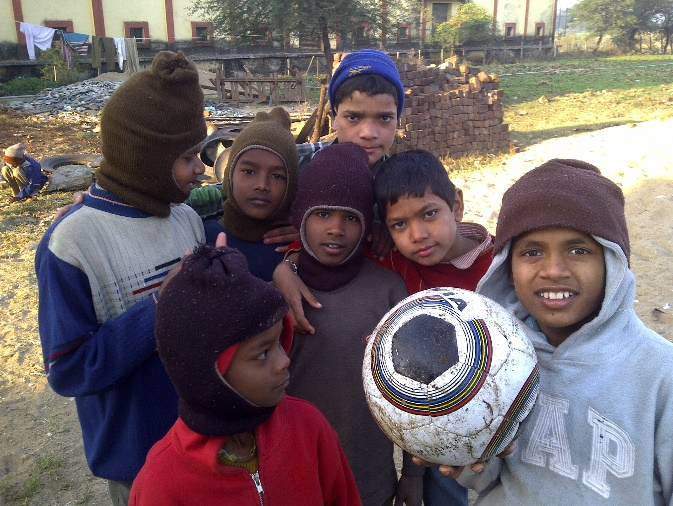
\includegraphics[height=3in]{Happykids}
  %   \caption{Children enjoying their time}
  %   \label{FigAir}
  % \end{center}

	\begin{subfigure}{.5\textwidth}
	  	\centering
	  	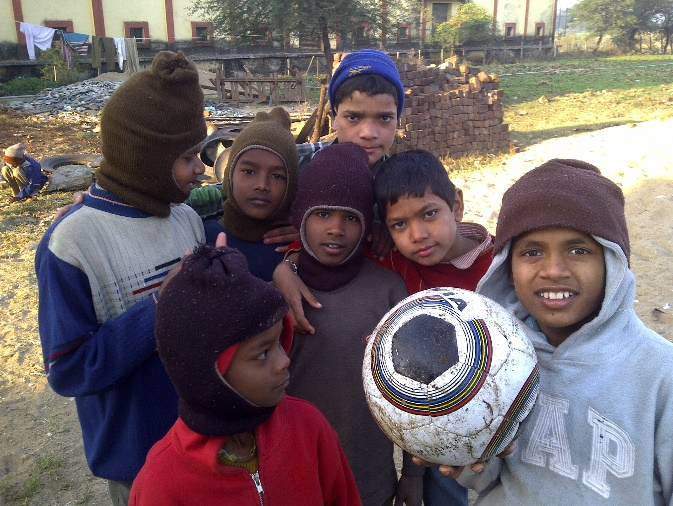
\includegraphics[width=2.6in]{Happykids}
	  	\caption{Children Enjoying their time}
	  	\label{fig:sub1}
	\end{subfigure}%
	\begin{subfigure}{.5\textwidth}
	  	\centering
	  	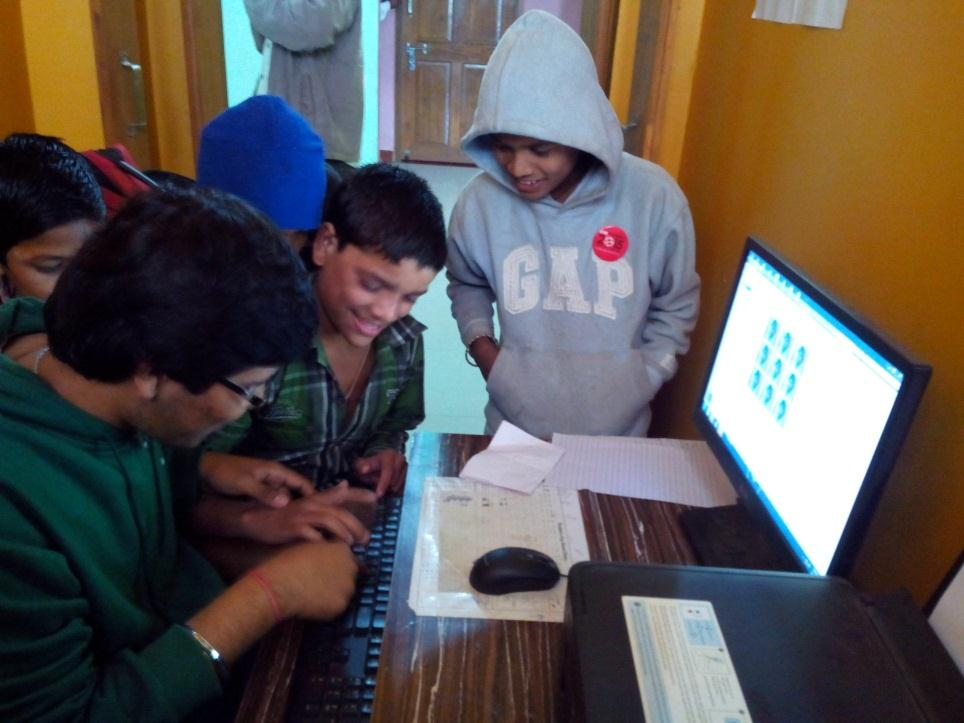
\includegraphics[width=2.6in]{Computer}
	  	\caption{Kids trying things on computer}
	  	\label{fig:sub2}
	\end{subfigure}
	\caption{Child line work}
	\label{figstart}
\end{figure}

\section{Villages}
Synergy Sansthan has brought remarkable changes in the rural areas. There is a small tribal village named ``Umardha'' 20 kms away from Harda. The village was originally in a pitiable state. Vishan Devda, a young man from Umardha started working at Synergy Sansthan. He then served the role of the middleman in communication between the Sansthan and the villagers. Together they set up a self help group for the women of the village. The self help group initially just collected money and gave small loans to the villagers. Later they started a bus service which would run buses from neighboring villages till Bhopal and Indore easing transportation for the people. They faced a lot of difficulties in this. Synergy Sansthan helped in doing all the legal work for establishing the SHG and also gave them support and guidance. Now those women are truly independent and are prospering. They have started adding more members to the group from different close by villages.

\begin{figure}[ht!]
	\begin{subfigure}{.5\textwidth}
	  	\centering
	  	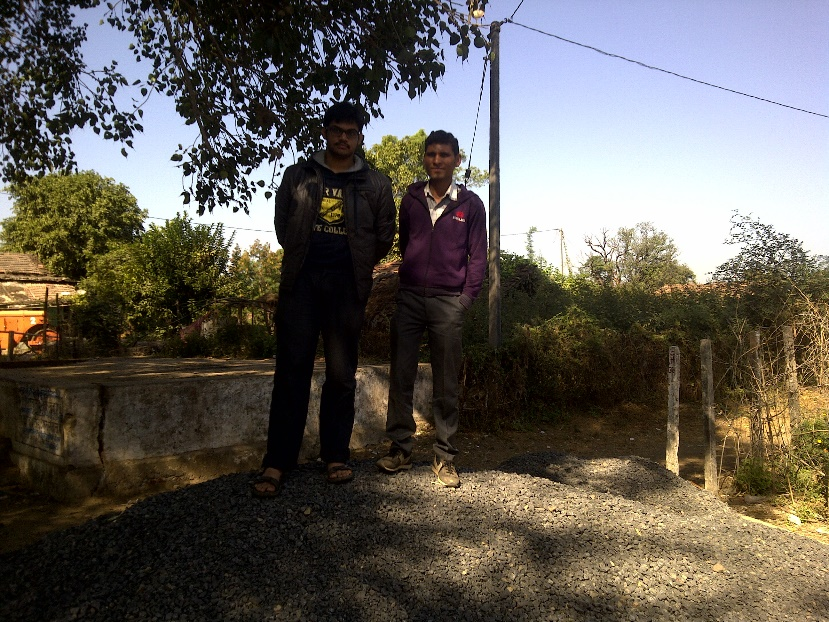
\includegraphics[width=2.6in]{withvishan}
	  	\caption{With Vishan (Representative)}
	  	\label{fig:sub1}
	\end{subfigure}%
	\begin{subfigure}{.5\textwidth}
	  	\centering
	  	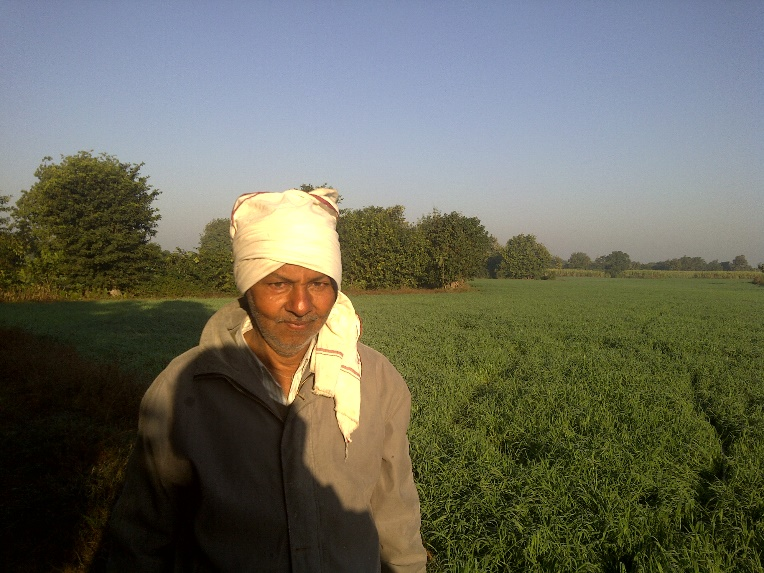
\includegraphics[width=2.6in]{vellagefarmer}
	  	\caption{Farmer in the village}
	  	\label{fig:sub2}
	\end{subfigure}
	\caption{Work Done in Villages}
	\label{figstart}
\end{figure}


Apart from this, it also helps the farmers. It takes the soil samples and gets them tested at the facilities in Harda. Then they communicate the fertilizers and manure needed for proper production of crops.

\section{Entrepreneurship development program}
The entrepreneurship development program was a bold initiative taken by Synergy Sansthan. It was with the help of partner NGO ``Pravah'' which is based in Delhi. It faced very low response rate initially because people were not attracted by it. Ajay sir took a lot of training in this so that he can mobilize people effectively and gradually they saw success. The number of people registering for this increased and the numbers of dropouts reduced. The people who have been through it have successfully received loans from banks and have all their paperwork in order. They are now better equipped to make their business grow. 
\begin{figure}[ht!]
	\begin{subfigure}{.5\textwidth}
	  	\centering
	  	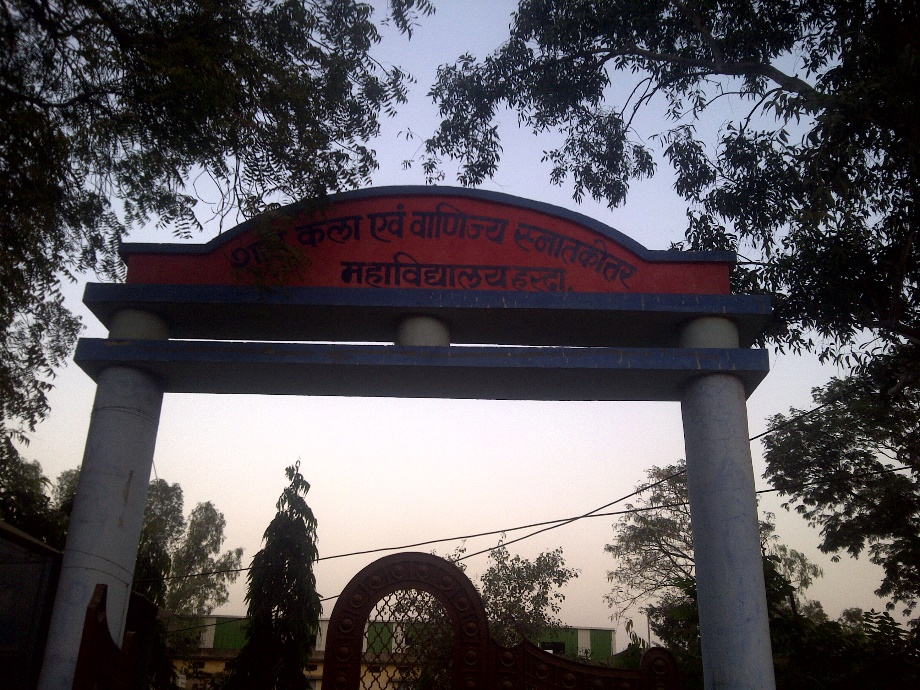
\includegraphics[width=2.6in]{college}
	  	\caption{Harda College}
	  	\label{fig:sub1}
	\end{subfigure}%
	\begin{subfigure}{.5\textwidth}
	  	\centering
	  	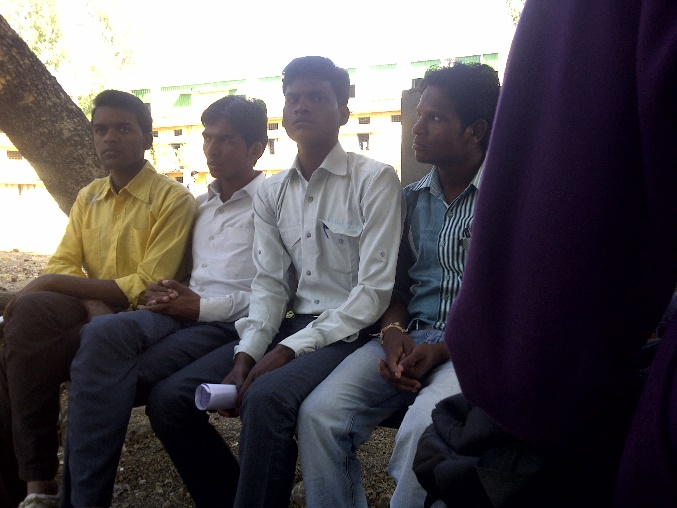
\includegraphics[width=2.6in]{members}
	  	\caption{Active participants of EDP}
	  	\label{fig:sub2}
	\end{subfigure}
	\caption{EDP Work}
	\label{figstart}
\end{figure}




% \subsection{first subsection in the Second Section}
% ... and some more ...

% \subsection{second subsection in the Second Section}
% ... and some more ...

% \subsection{third subsection in the Second Section}
% ... and some more ...


% ------------------------------------------------------------------------

%%% Local Variables: 
%%% mode: latex
%%% TeX-master: "../thesis"
%%% End: 
